\chapter{Signature of the Signal}
\label{cha:sig}

As discussed in section~\ref{sec:anamodel}, the model used in the analysis is $R$-parity violating supersymmetry. In particular, single coupling dominance for the lepton number violating coupling $\lambda^\prime_{211}$ is assumed. With a two quark initial state, the production of sleptons inevitably dominates other constellations. Considering how the low values for the couplings have to be (C.f.~fig.~\ref{fig:auterrpv}~\&~\ref{fig:endresrpv}), the primary decay modes for the slepton will be the $R$-parity \textit{conserving} $\nu + \tilde{\chi}$ or $\mu + \tilde{\chi}$ combination. The $R$-parity \textit{violating} dijet channel be neglected as it will be both rare and overshadowed by standard model processes. The lightest neutralino is assumed to be the lightest supersymmetric particle (\textbf{LSP}) in this analysis. As a result the decay products of both the neutralino and chargino can lead to additional jets or leptons, but will eventually lead to the lightest neutralino through $R$-parity conserving modes\footnote{The details of the decay modes depend on the mass hierarchy determined by the RPV cMSSM model parameters}. 


Since it is the LSP, it can only decay through the $\lambda^\prime_{211}$ coupling via a virtual smuon or sneutrino. It should also be noted that the lifetime of the LSP depends on the coupling strength. For values larger than $\lambda^\prime_{211} > 10^{-6}$, the decay will be perceived as ``prompt'' by the detector. This means that both muons should originate from the same (primary) vertex. This decay subsequently adds two jets, as well as either a muon or neutrino. With missing transverse energy from neutrinos being significantly less attractive than muon signatures, these final states are being neglected. 


This leaves two guaranteed jets and a variable amount of muons, ranging from zero to two, in every decay. Considering the production rates for the relevant backgrounds, one can see that two compositions are disfavoured. Colliding two hadrons yields a high amount of jets in every event, making the pure dijet channel without any muon the least promising. The very high $W + \text{jets}$ background would interfere with a single muon with two jet search, leaving only the two muon, two jets option. Even here there are significant backgrounds to reduce, primarily the Drell-Yan processes.

Taking a look at the most simple Feynman graphs for resonant smuon and sneutrino production at the LHC (Fig.~\ref{fig:resosmusneu}), one will notice a very useful attribute of their decay products.

\begin{figure}[ht!]
  \centering
  \begin{subfigure}[b]{0.495\textwidth}
    \centering
    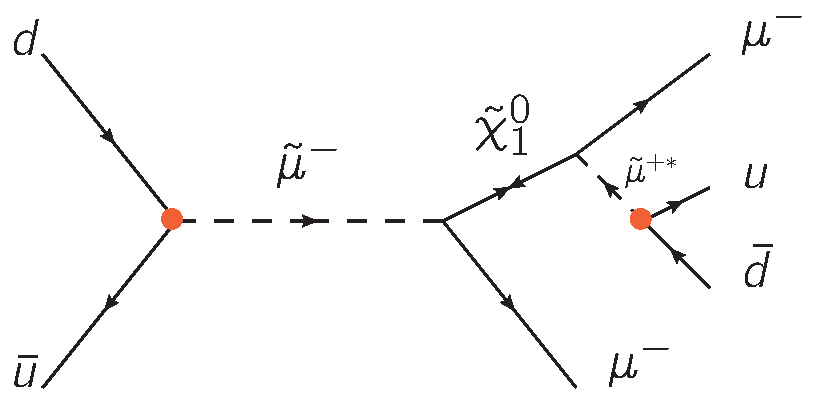
\includegraphics[width=\textwidth]{plots/rpv-resonant-smuon-samesign-mumuqq.pdf}
    \caption{\label{fig:ressmu}}
  \end{subfigure}
  \begin{subfigure}[b]{0.495\textwidth}
    \centering
    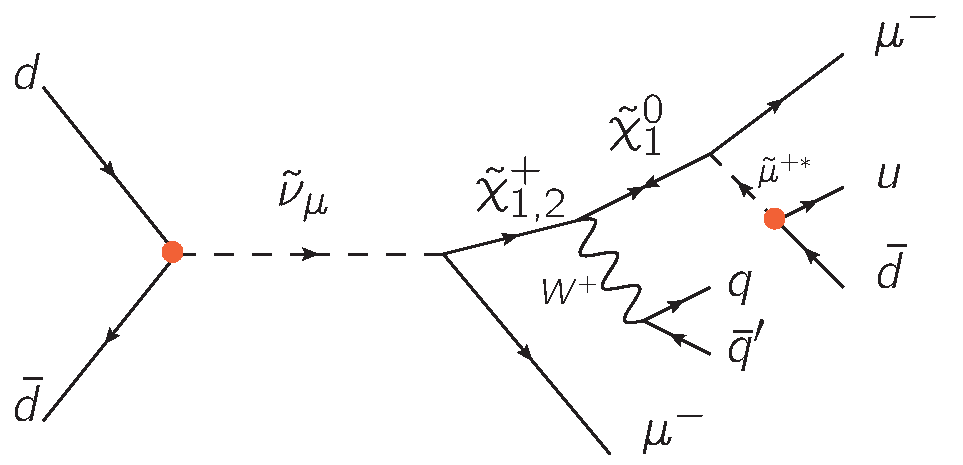
\includegraphics[width=\textwidth]{plots/rpv-resonant-sneutrino-chargino-mumuqq.pdf}
    \caption{\label{fig:ressneu}}
  \end{subfigure}
  \caption{Resonant production of a smuon~(\ref{fig:ressmu}) and a sneutrino~(\ref{fig:ressneu}) in $R$-parity violating supersymmetry. Shown are the most simple Feynman graphs leading to the two muon, two jets final state. The lepton number violating vertices are marked in red.}
  \label{fig:resosmusneu}
\end{figure}

\noindent The electric charge of both muons are equally as likely to have the same sign as the opposite sign. This is due to the neutralino being a Majorana particle. Keeping the initial state of two protons in mind, primarily the ratio of $u$ to $d$-quarks, the likelihood of positively charged muons is twice as high as the one for negatively charged ones. Since most Standard Model backgrounds are able to produce two opposite, but not two same sign muons, this feature of RPV supersymmetry can be exploited to discriminate against them. Major backgrounds, such as the aforement Drell-Yan processes or the production of top quark pairs, can be greatly reduced, enabling searches for new physics with low cross sections.


\section{Monte Carlo Study}
\label{sec:mcstudy}

As Monte Carlo (\textbf{MC}) simulations are used for comparison to the measured data, the simulation of the signal for the 2011 analysis~\cite{endres} can be repurposed to derive further information about the signature. The production process of such a simulation will be outlined in an upcoming section (Sec.~\ref{sec:mcstudy}). Using the RPV supersymmetry model explained in section~\ref{sec:anamodel}, a grid of simulations with $50\,\text{k}$ events each has been generated. While the mass of the scalar sparticles $m_0$ runs from $100$ to $2000\,\text{GeV}$ in steps of $100\,\text{GeV}$ and the mass of fermionic sparticles runs from $50$ to $1000\,\text{GeV}$ in steps of $50\,\text{GeV}$, the remaining model parameters have the following set values:

\begin{equation*}
  A_0 = 0, \quad \tan{\beta} = 20, \quad \text{sgn}\,\mu = +1, \quad \lambda^\prime_{211} = 0.01
\end{equation*}

Because certain regions (low $m_{1/2}$, high $m_0$) in this parameter space lead to unphysical phenomena such as non-converging renormalization group equations, the existence of tachyons or no electroweak symmetry breaking, they are not being simulated. Excluding these points in the grid leaves an overall amount of $354$ simulations (C.f.~fig.~\ref{fig:sigeff}). \\

Various decay scenarios have been searched for in this grid to determine their respective contribution to the signal signature. These searches have been performed under consideration of two cases. In the first one a minimum of both two muons and two jets are required (\textbf{MU2J2}). This yields signal-like, but not necessarily signal events. The second one demands all analysis requirements (from 2011) to be met (\textbf{ANA}). While it is important to know that the latter is more strict than the first, the details of all the requirements will be discussed in-depth in the event selection\footnote{Although the event selection will concern itself with the 2012 requirements, they are comparable to the ones used in 2011.} (Cha.~\ref{cha:eventsel}). Comparing both types of cases gives an idea of the effect of the analysis requirements on the signal.

To determine the overall efficiency of selecting signal-like events, only the MU2J2 and ANA cases without any specific decay scenario are shown in figure~\ref{fig:sigeff}.

\begin{figure}[ht!]
  \centering
  \begin{subfigure}[b]{0.495\textwidth}
    \centering
    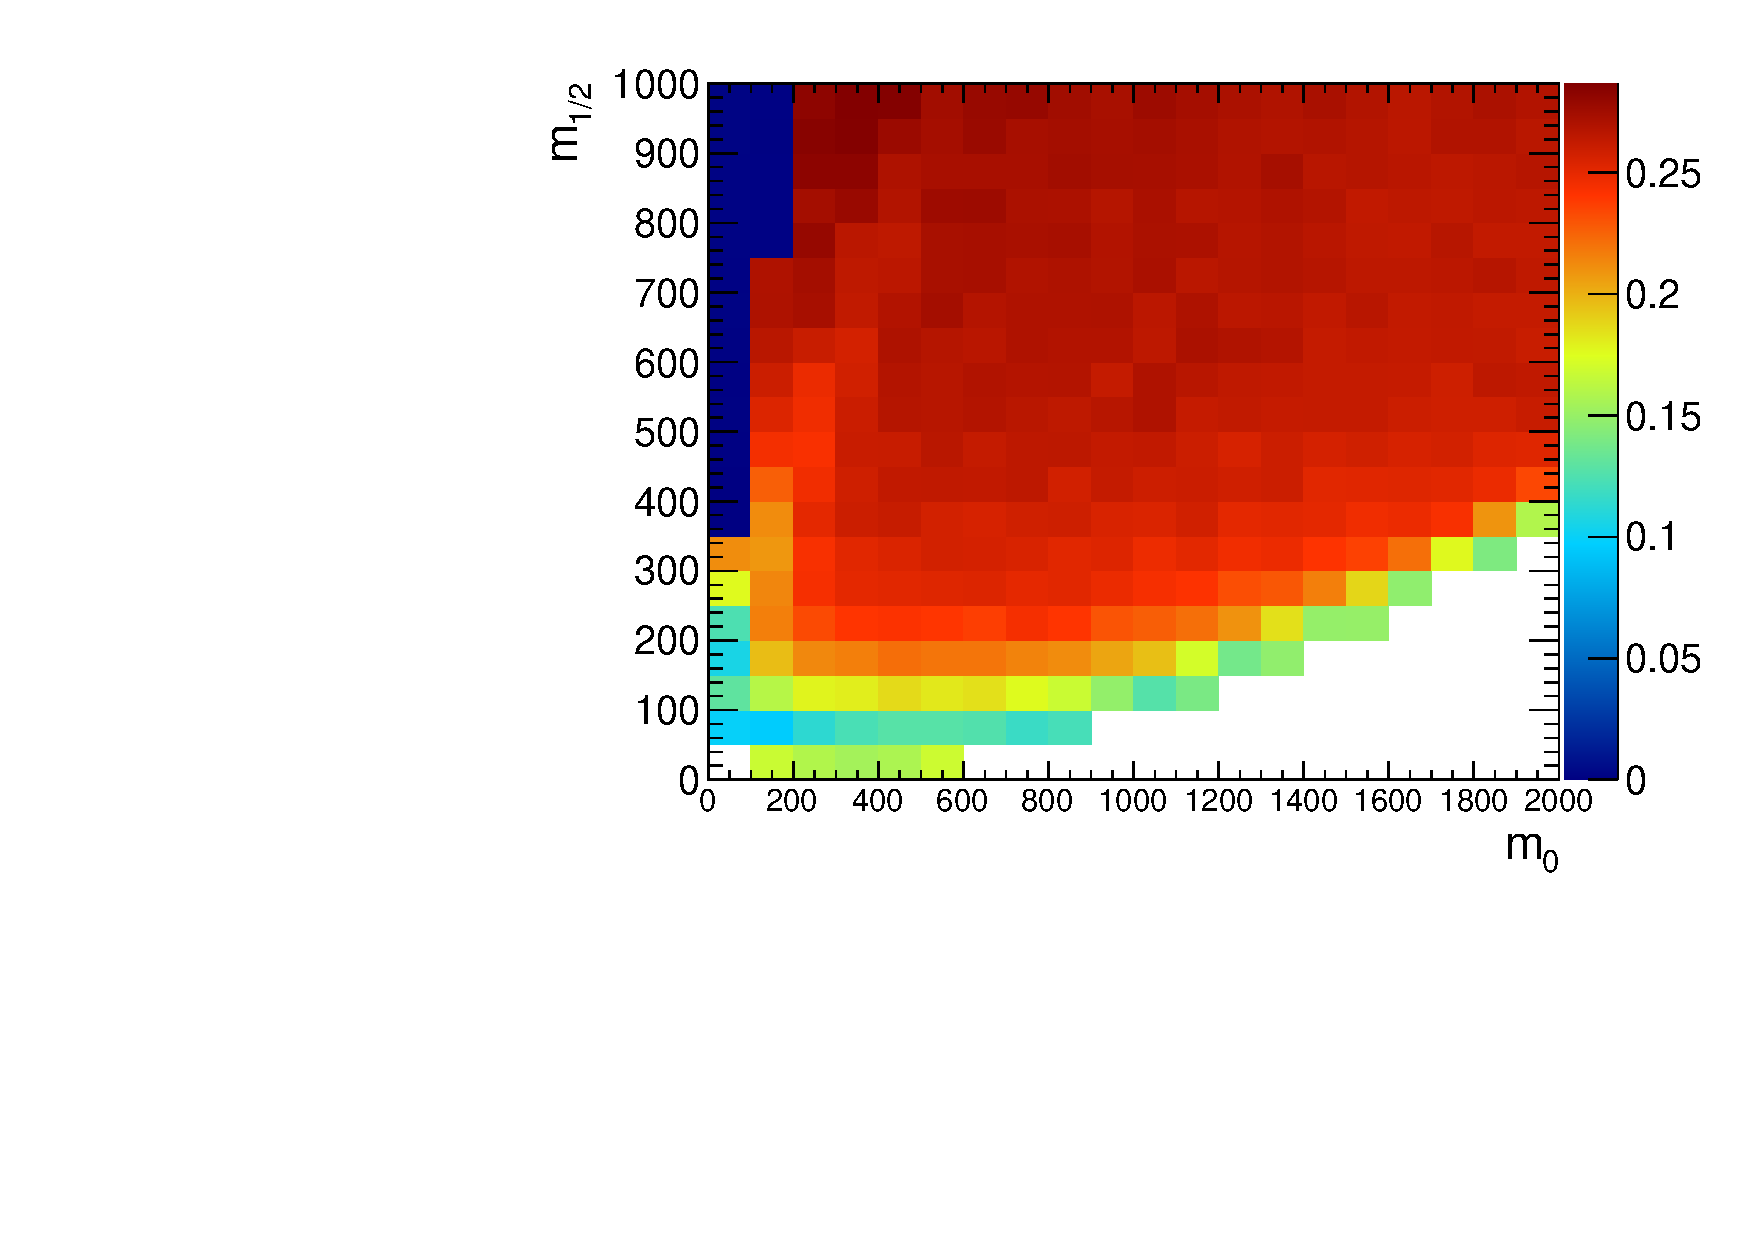
\includegraphics[width=\textwidth]{plots/hSignalRatio.pdf}
    \caption{\label{fig:sig}}
  \end{subfigure}
  \begin{subfigure}[b]{0.495\textwidth}
    \centering
    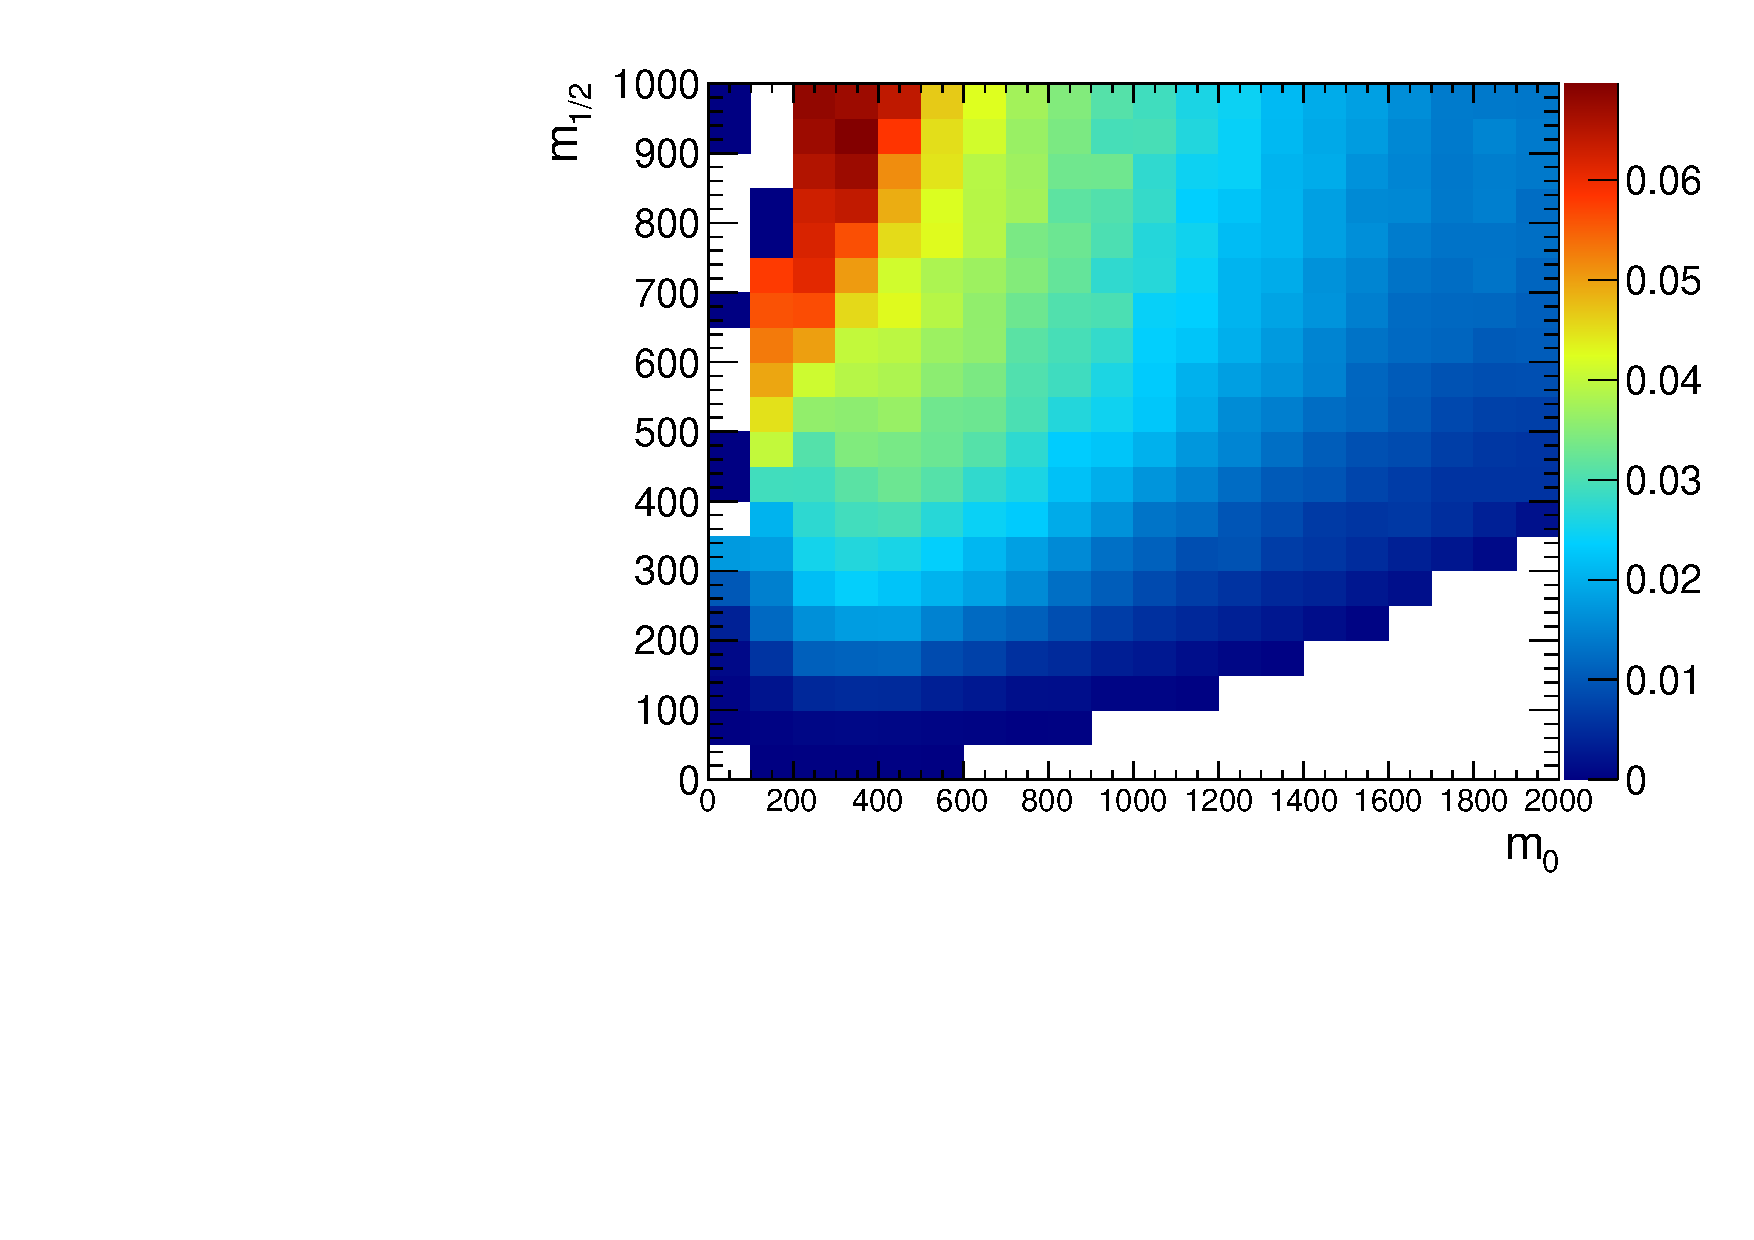
\includegraphics[width=\textwidth]{plots/hCutSignalRatio.pdf}
    \caption{\label{fig:cutsig}}
  \end{subfigure}
  \caption{Efficiency of selecting signal(-like) events are shown in the MU2J2~(\ref{fig:sig}) and the ANA case~(\ref{fig:cutsig}). Each bin represents a Monte-Carlo simulation of a RPV supersymmetry model normalized to the generated number of events.}
  \label{fig:sigeff}
\end{figure}

\noindent Each bin shows the number of events meeting the requirements, normalized to the generated number of events. The white bins contain no events. This is either because no events passed the requirements, or they are within the previously mentioned low $m_{1/2}$, high $m_0$ parameter region with unphysical results. For high $m_{1/2}$, but low $m_0$ there are also disproportionally few events. The reason for this disparity lies within the supersymmetric mass spectrum. The lightest supersymmetric particle changes from the lightest neutralino to the stau $\tilde{\tau}$. As a result, the decay chains are altered, therefore rendering the analysis requirements insensitive. 

Shifting the focus on the shape of the distribution, one will notice an almost flat efficiency of around $25\,\pct$ above a certain ratio of $m_{1/2}$ to $m_0$ in the MU2J2 case. However, adding the ANA requirements leads to an efficiency decline from the $\sim 6\,\pct$ high $m_{1/2}$, low $m_0$ region to either around or below $1\,\pct$ for increasing $m_0$ and $m_{1/2}$, respectively. A significant portion of the drop in efficiency is expected when using the ANA case. As discussed in the previous section, the additional same sign charge requirement will half the selected amount of events already. Any further requirements will also have a negative impact on the efficiency, with the isolation criteria for the two muons being the main cause for the decline. If the neutralino masses are much lower than the smuon mass, which is directly related to the universal mass parameters, it will naturally lead to boosted particles in the decay. Should these decay products be too collimated, the isolation criteria will not be met and the event will be discarded. It should be noted that, as a result of different branching ratios in certain phase space regions, different processes can dominate the final state. Consequently the requirements of the ANA case cannot impact the entire phase space equally. Therefore the origin of the decline is always a composite of multiple quantities. \\

By demanding certain amounts of specific particles in a decay chain, it possible to reconstruct the process of a selected event. To get an overview of the composition of processes leading to the signal signature, the particle count has been varied systematically. To reduce redundancy, only the primary produced sparticle as well as its supersymmetric decay products are used for process identification. Upon reaching the neutralino LSP in the cascade, the decay through the $\lambda^\prime_{211}$ coupling is always identical.

\begin{figure}[ht!]
  \centering
  \begin{subfigure}[b]{0.495\textwidth}
    \centering
    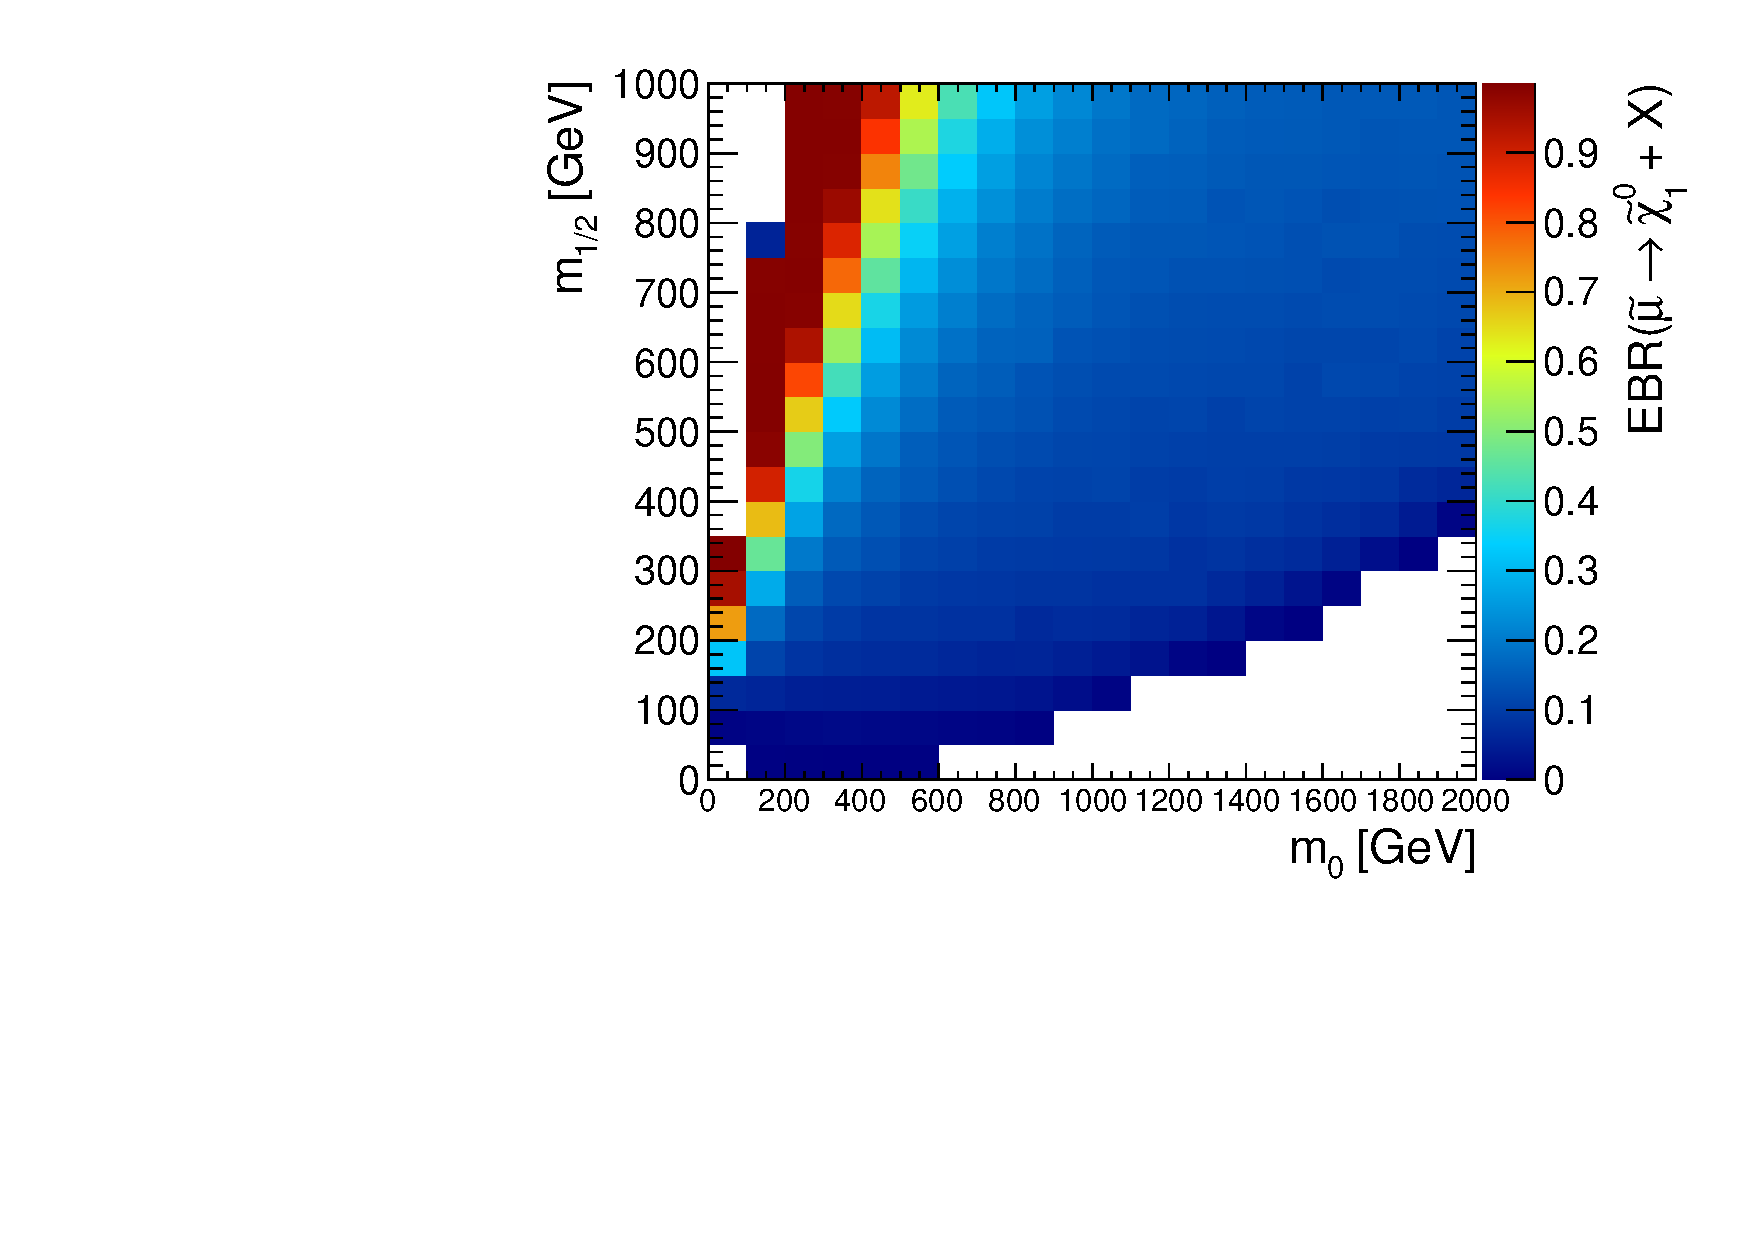
\includegraphics[width=\textwidth]{plots/hX01Ratio.pdf}
    \caption{\label{fig:x01}}
  \end{subfigure}
  \begin{subfigure}[b]{0.495\textwidth}
    \centering
    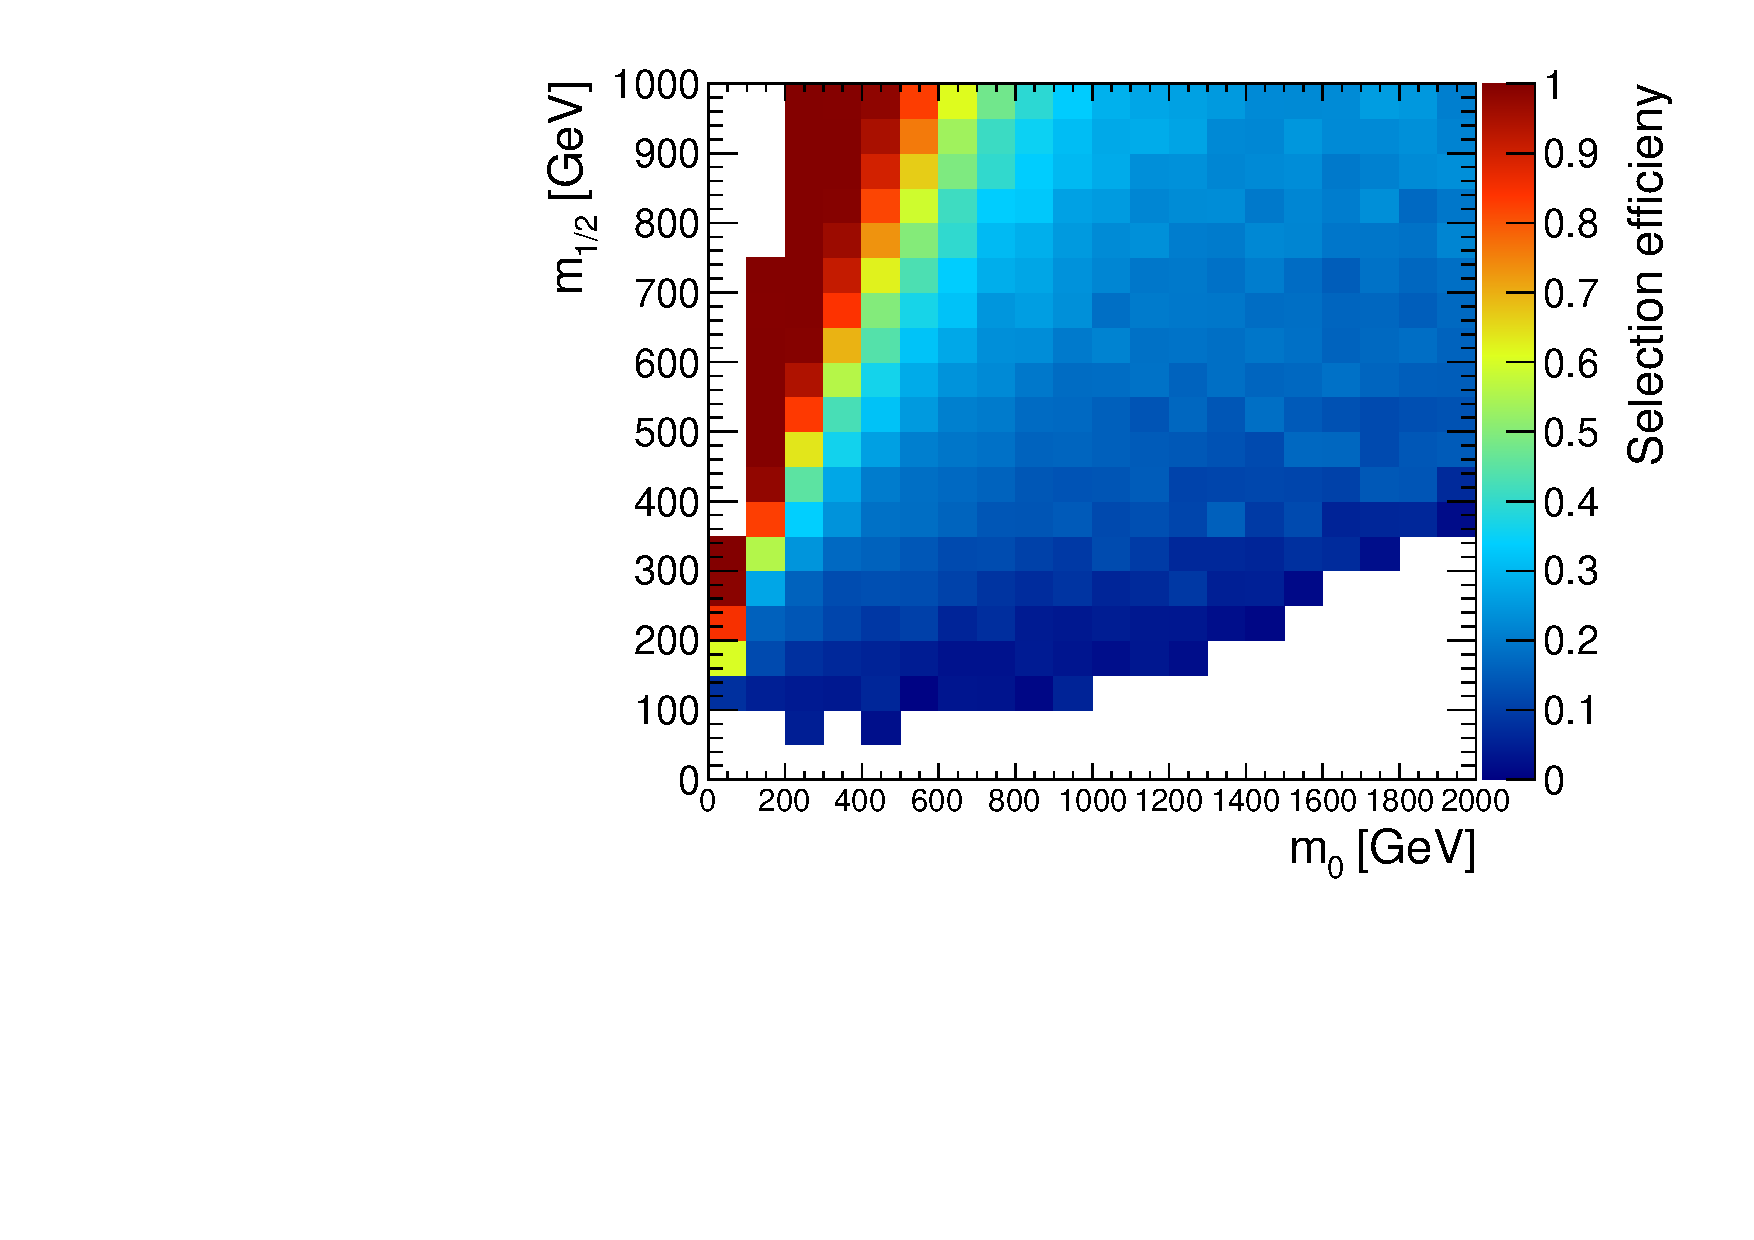
\includegraphics[width=\textwidth]{plots/hCutX01Ratio.pdf}
    \caption{\label{fig:cutx01}}
  \end{subfigure}

  \begin{subfigure}[b]{0.495\textwidth}
    \centering
    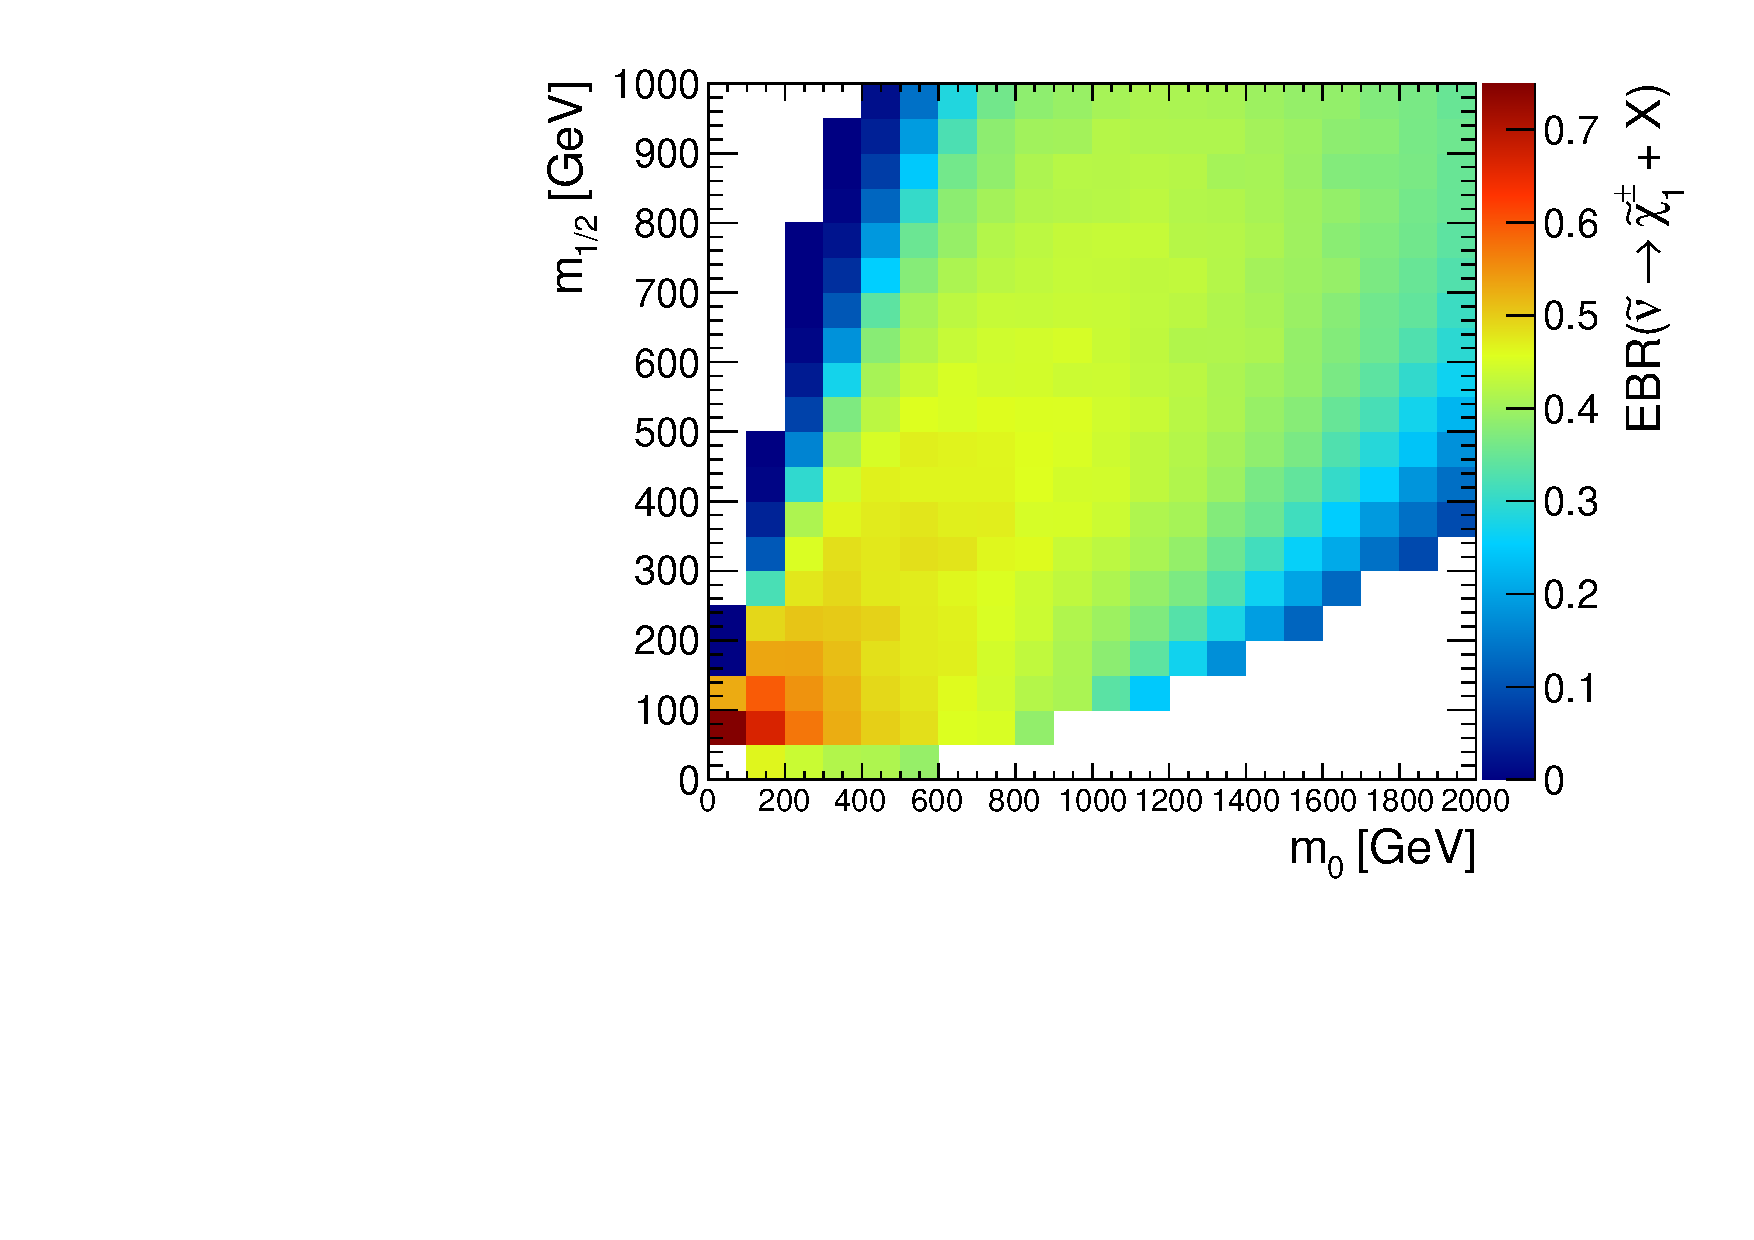
\includegraphics[width=\textwidth]{plots/hXplus1NeutRatio.pdf}
    \caption{\label{fig:xplus1neut}}
  \end{subfigure}
  \begin{subfigure}[b]{0.495\textwidth}
    \centering
    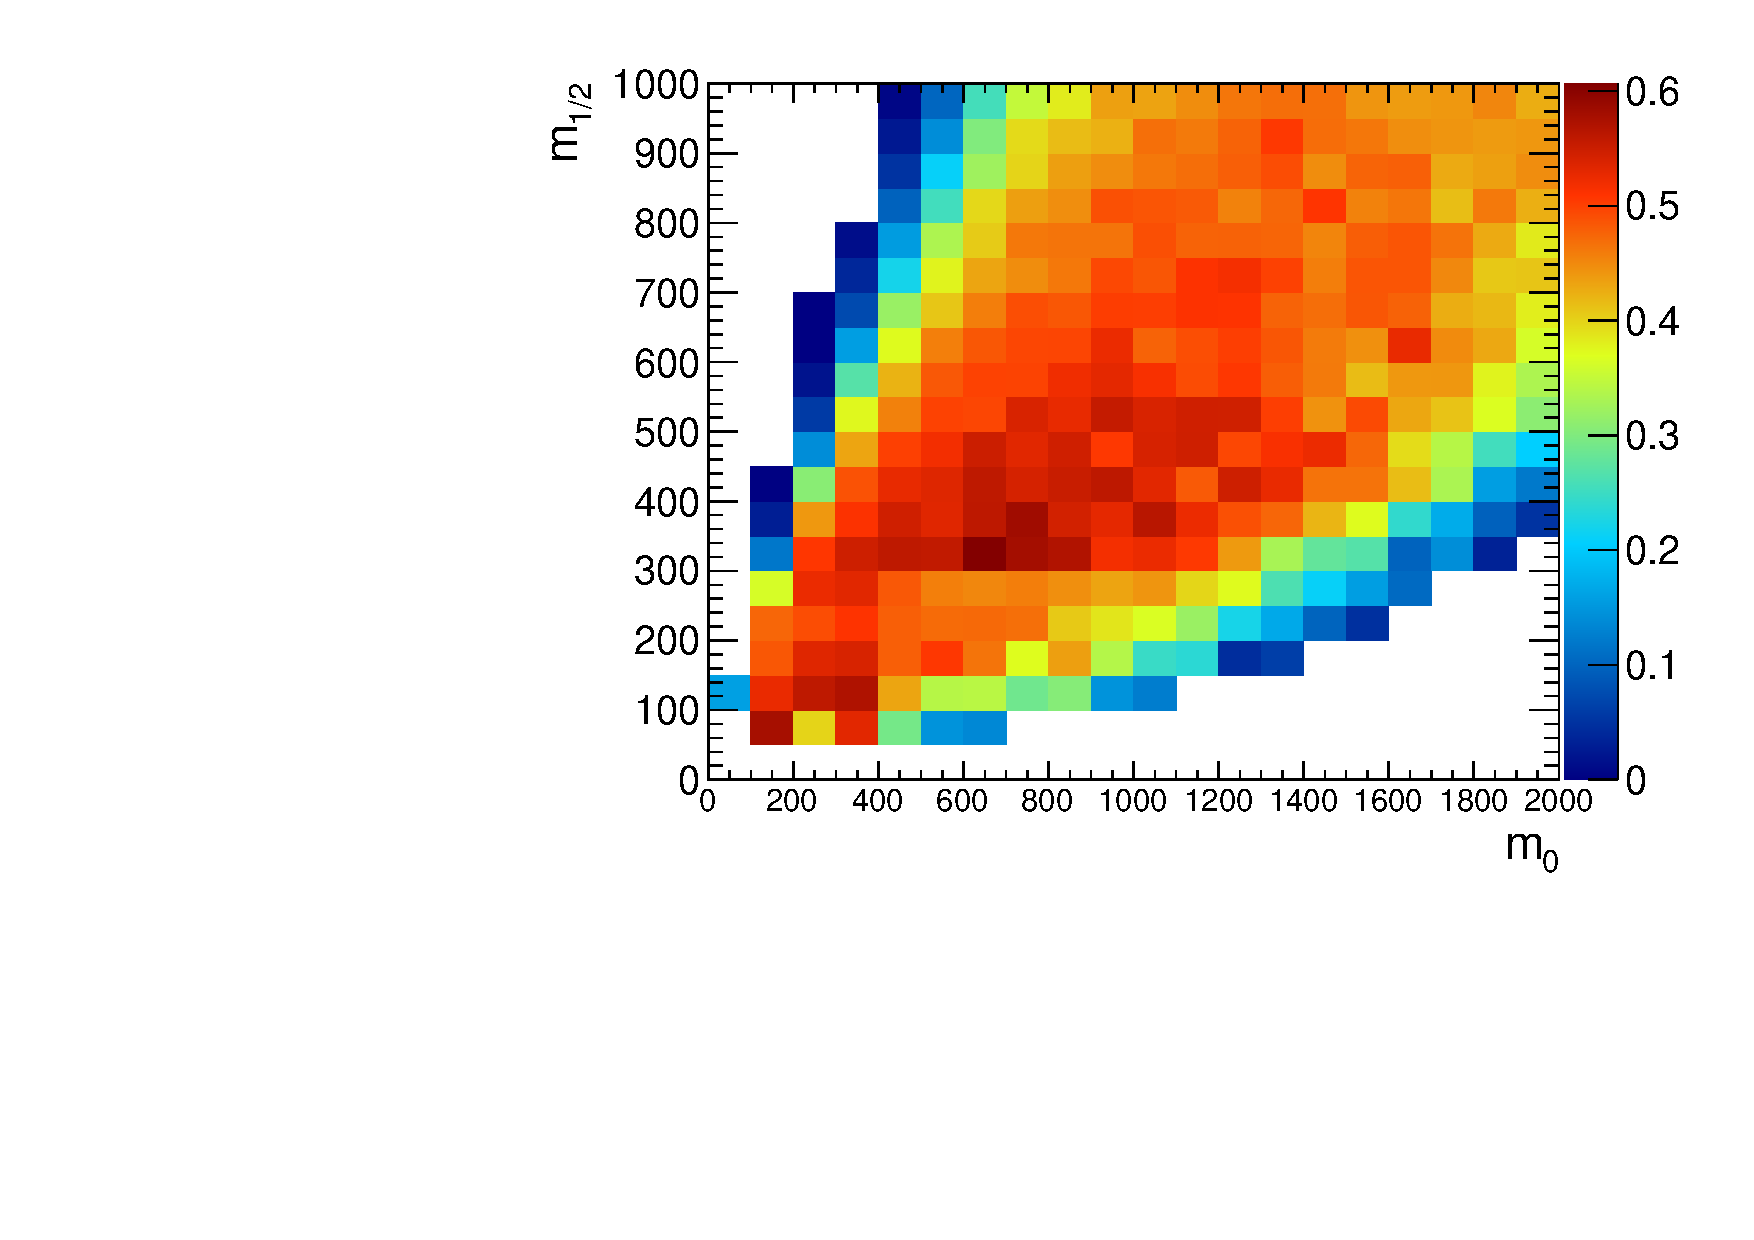
\includegraphics[width=\textwidth]{plots/hCutXplus1NeutRatio.pdf}
    \caption{\label{fig:cutxplus1neut}}
  \end{subfigure}
  \caption{Contributions to the selected signal(-like) events from figure~\ref{fig:sigeff} are shown for $\tilde{\mu} \rightarrow \tilde{\chi}^0_1$~(\ref{fig:x01}~\&~\ref{fig:cutx01}) and $\tilde{\nu} \rightarrow \tilde{\chi}^\pm_1$~(\ref{fig:xplus1neut}~\&~\ref{fig:cutxplus1neut}) processes. Both distributions on the left show the MU2J2 case, while the ANA case is given on the right side. Each bin represents a Monte-Carlo simulation of a RPV supersymmetry model divided by the respective bin content from~\ref{fig:sigeff}, thus representing their relative contribution.}
  \label{fig:x01sneuxplusratio}
\end{figure}

\noindent As an example, figure~\ref{fig:x01sneuxplusratio} displays the contributions of $\tilde{\mu} \rightarrow \tilde{\chi}^0_1$ and $\tilde{\nu} \rightarrow \tilde{\chi}^\pm_1$ processes. Combining these two processes already covers roughly $50\pct$ for most of the parameter space. An efficient way to compare all relevant processes at once, is a one dimensional distribution with either of the two universal mass parameters set to a fixed value. Since a larger variance can be observed over the simulated $m_0$ range (C.f. fig.~\ref{fig:sigeff}~\&~\ref{fig:x01sneuxplusratio}), $m_{1/2}$ is kept constant.

\begin{figure}[ht!]
  \centering
  \begin{subfigure}[b]{0.495\textwidth}
    \centering
    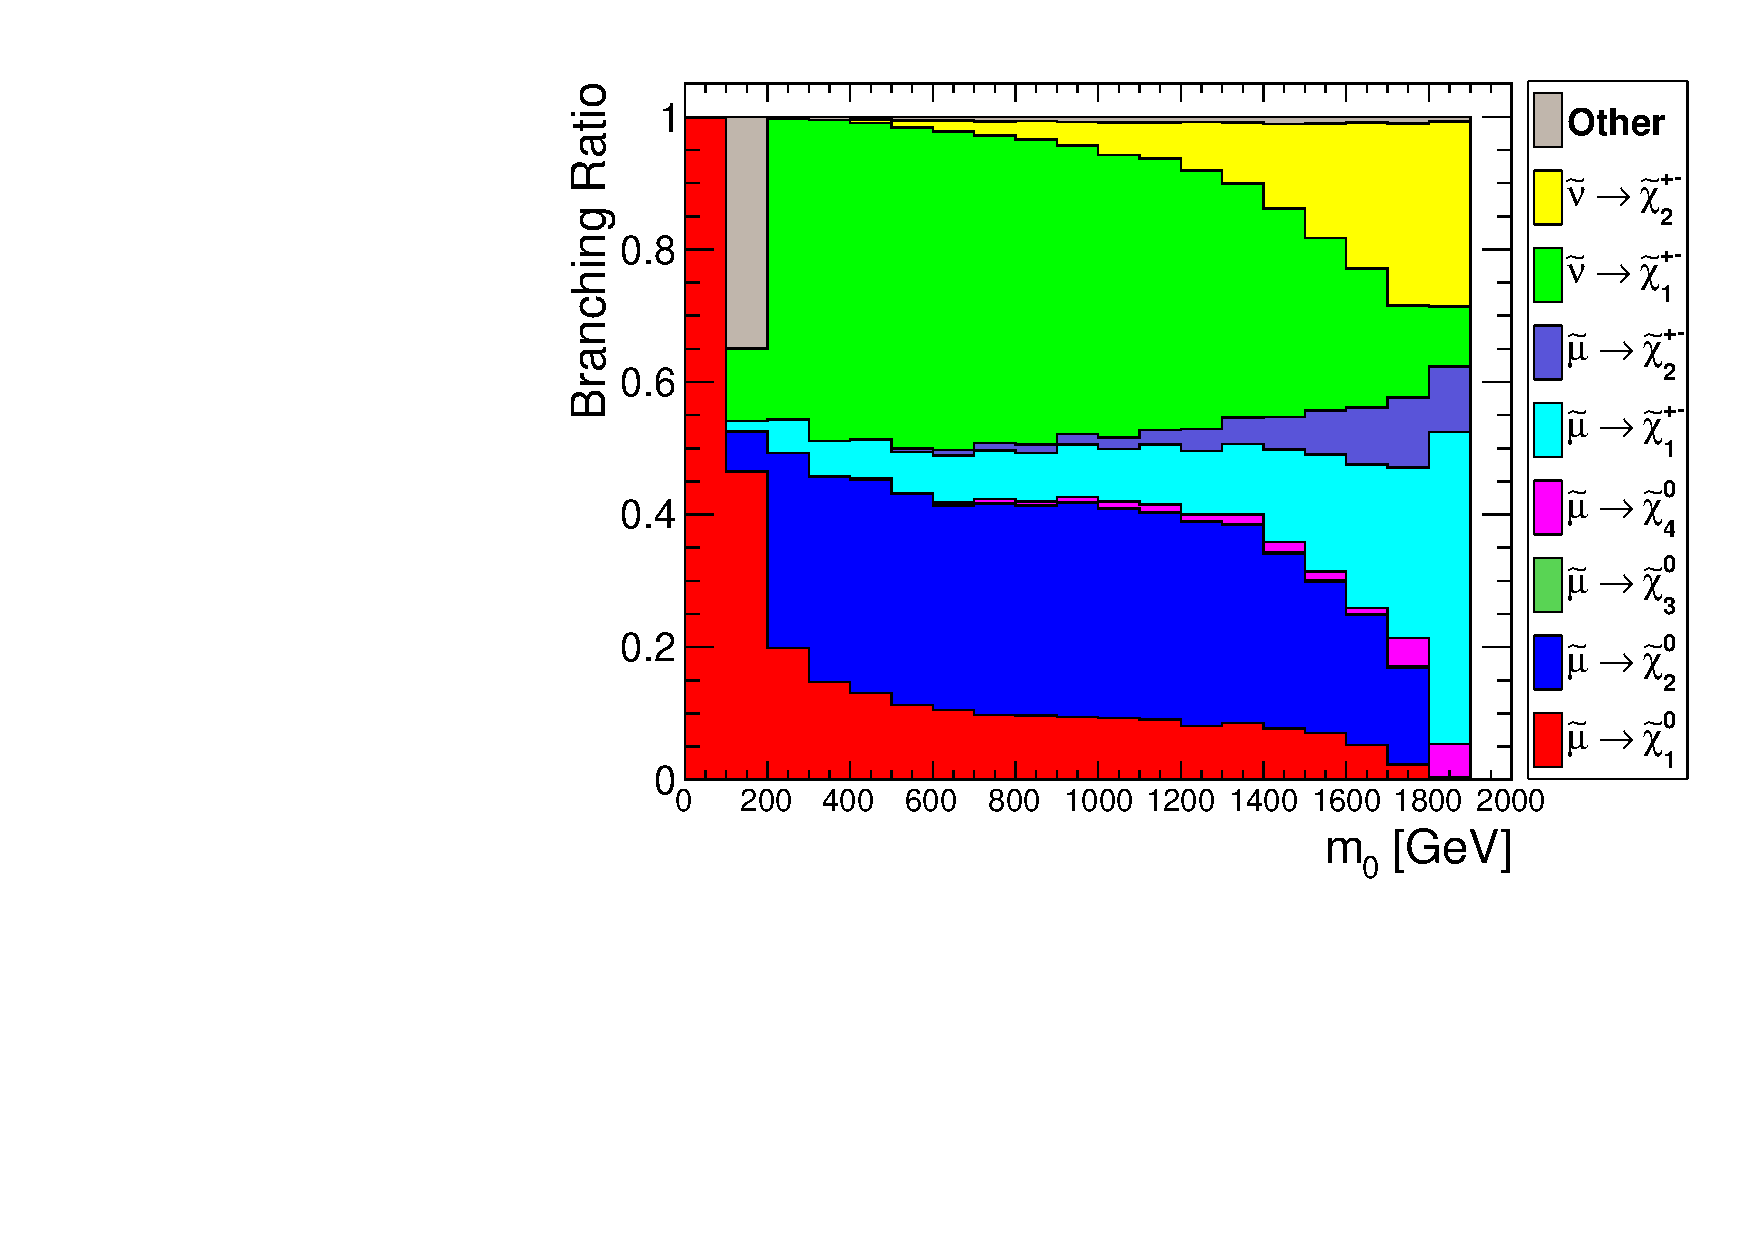
\includegraphics[width=\textwidth]{plots/hCrossRatio350.pdf}
    \caption{$m_{1/2} = 350\,\text{GeV}$\label{fig:crossratio350}}
  \end{subfigure}
  \begin{subfigure}[b]{0.495\textwidth}
    \centering
    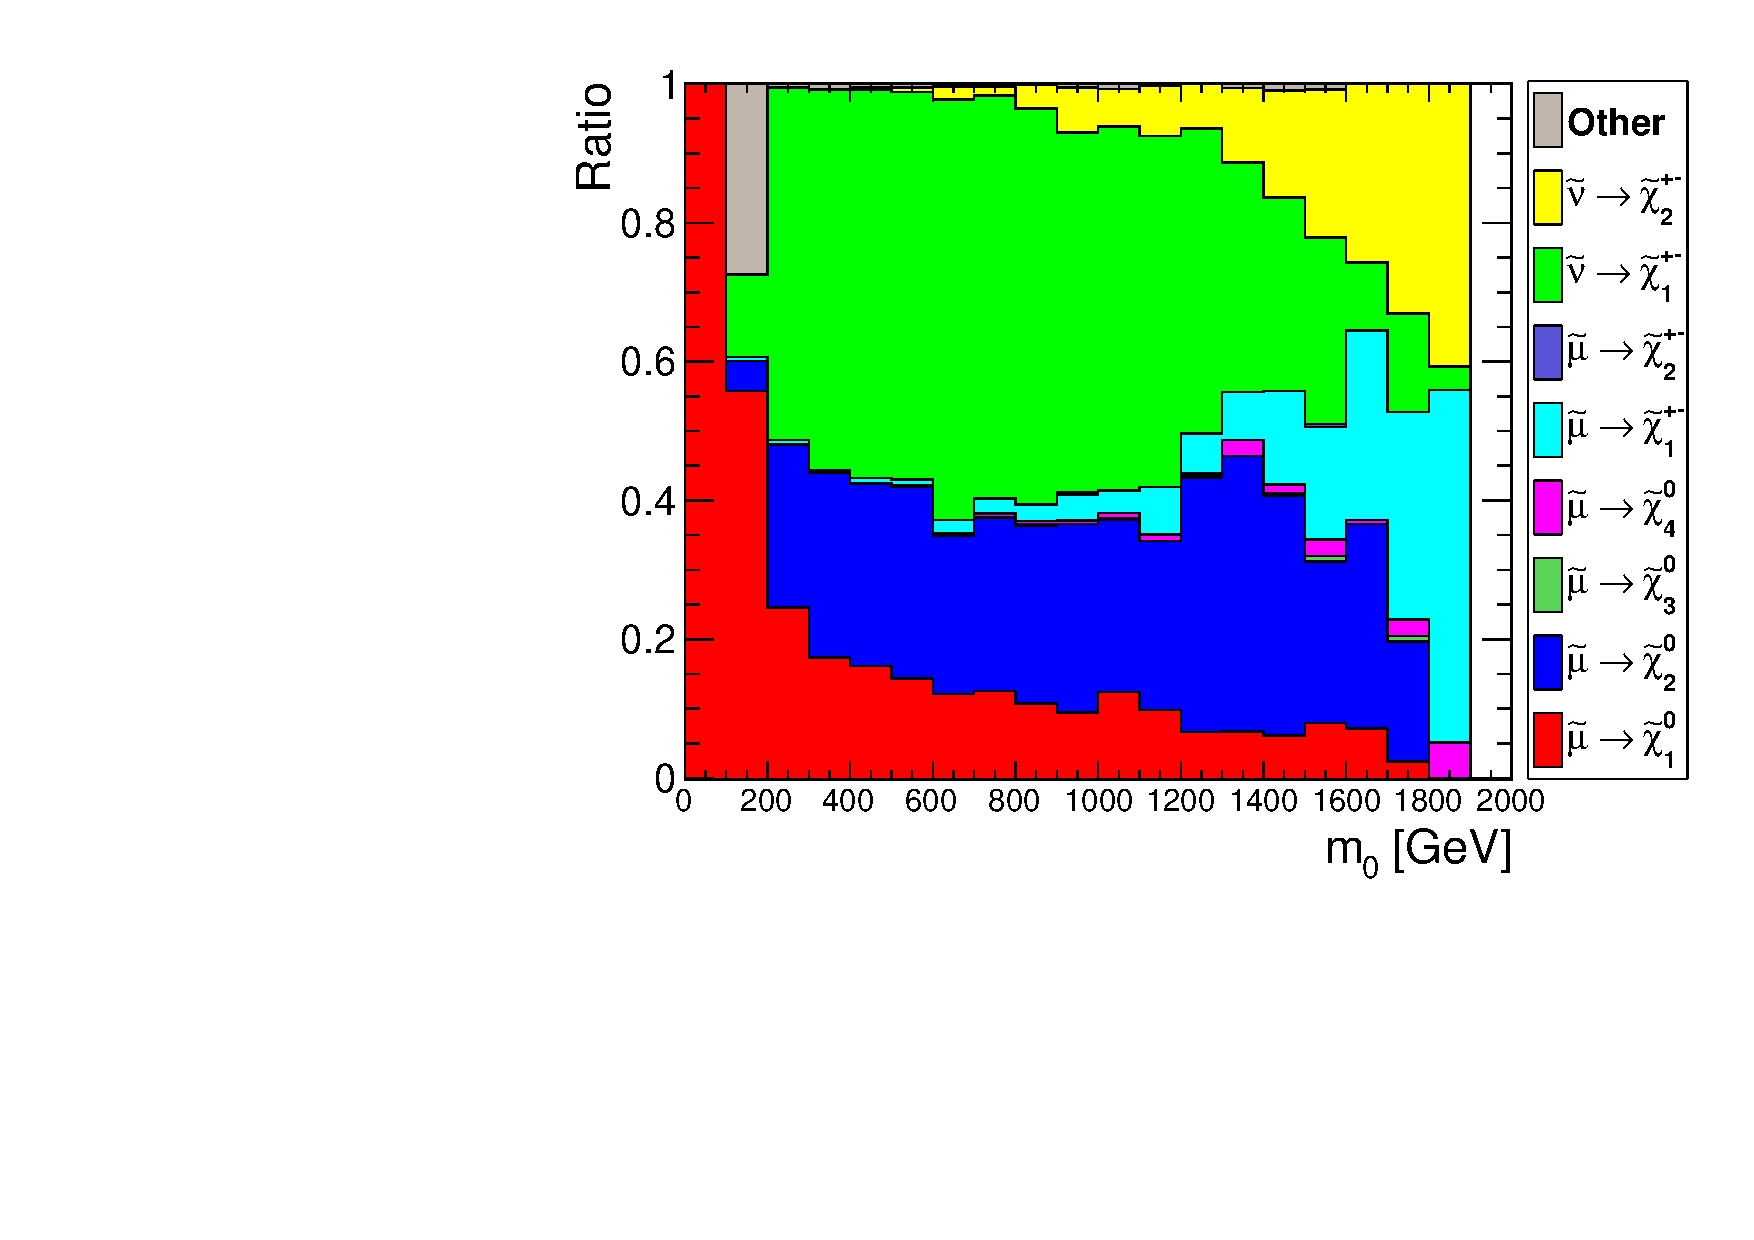
\includegraphics[width=\textwidth]{plots/hCutCrossRatio350.pdf}
    \caption{$m_{1/2} = 350\,\text{GeV}$\label{fig:cutcrossratio350}}
  \end{subfigure}

  \begin{subfigure}[b]{0.495\textwidth}
    \centering
    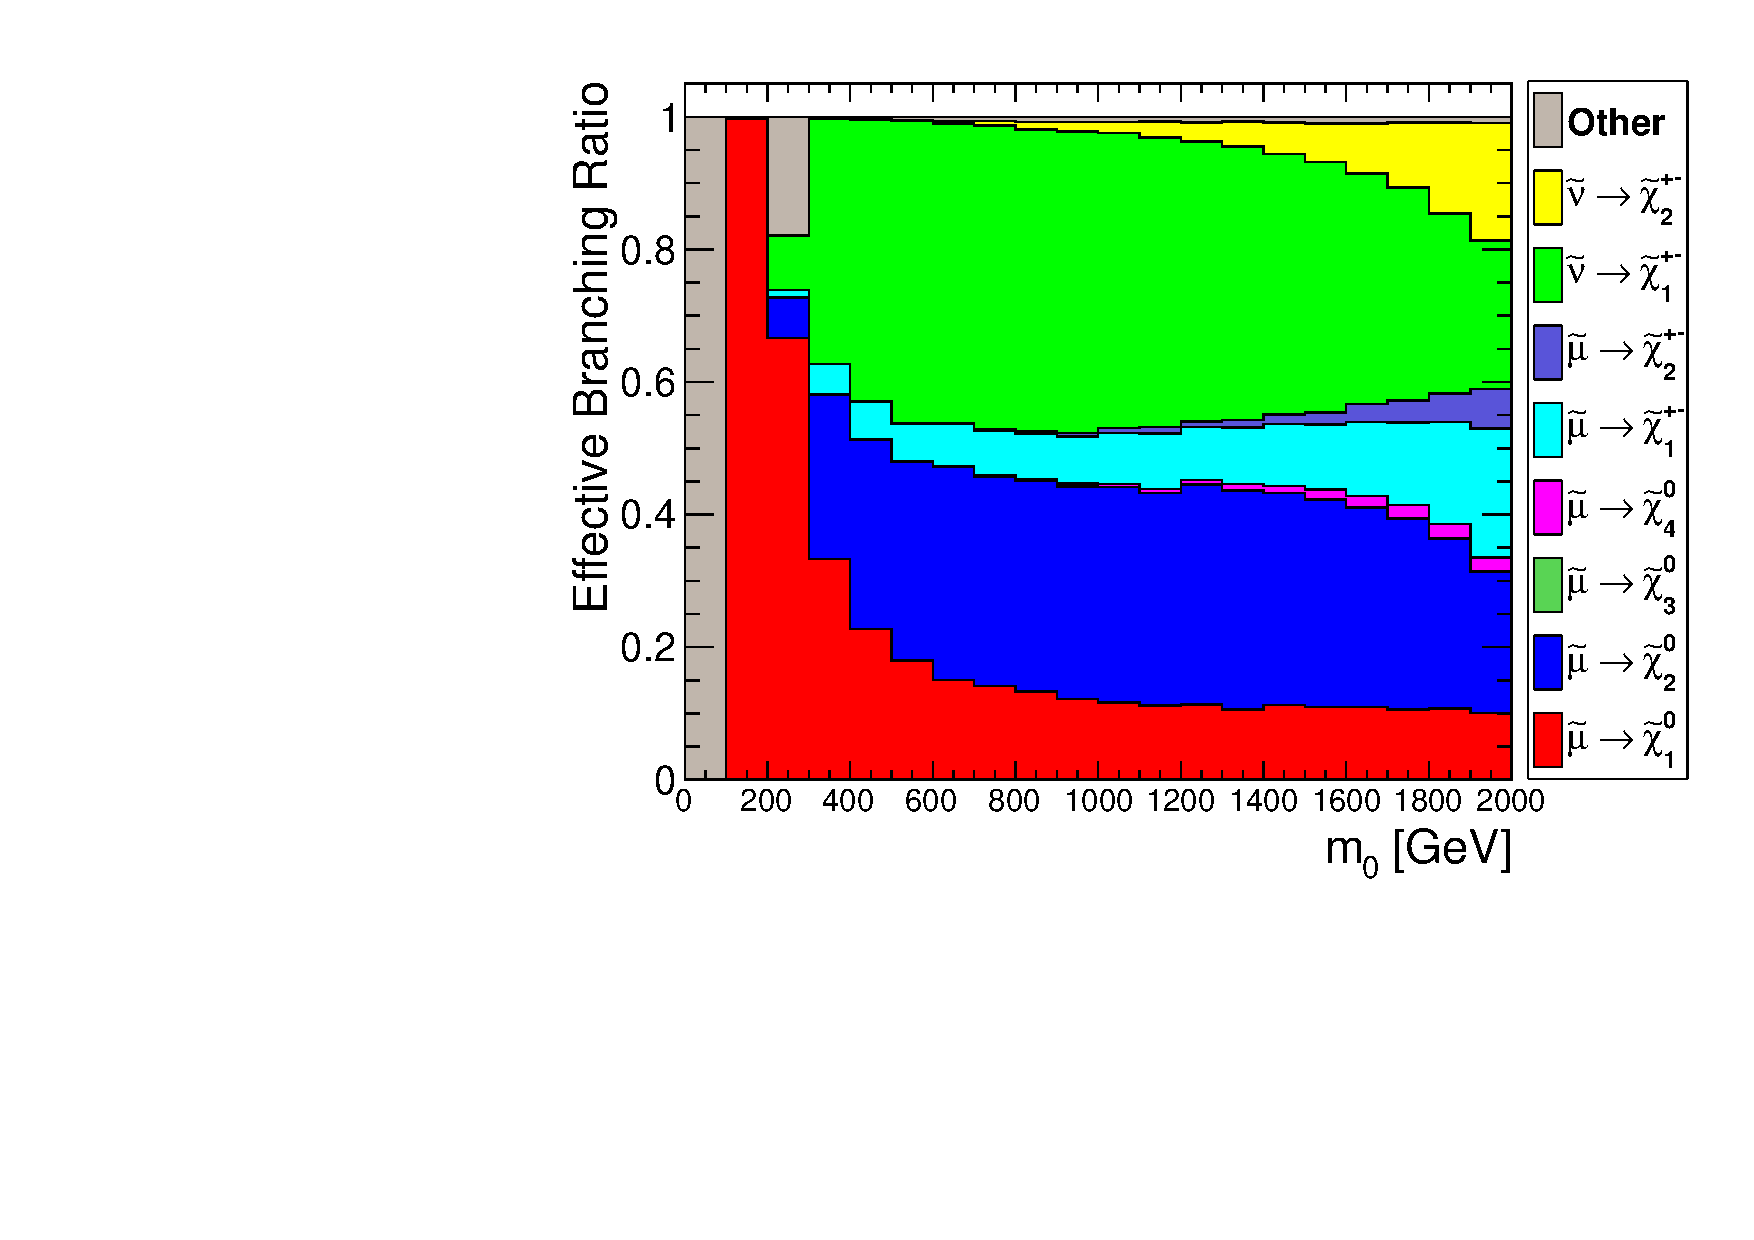
\includegraphics[width=\textwidth]{plots/hCrossRatio550.pdf}
    \caption{$m_{1/2} = 550\,\text{GeV}$\label{fig:crossratio550}}
  \end{subfigure}
  \begin{subfigure}[b]{0.495\textwidth}
    \centering
    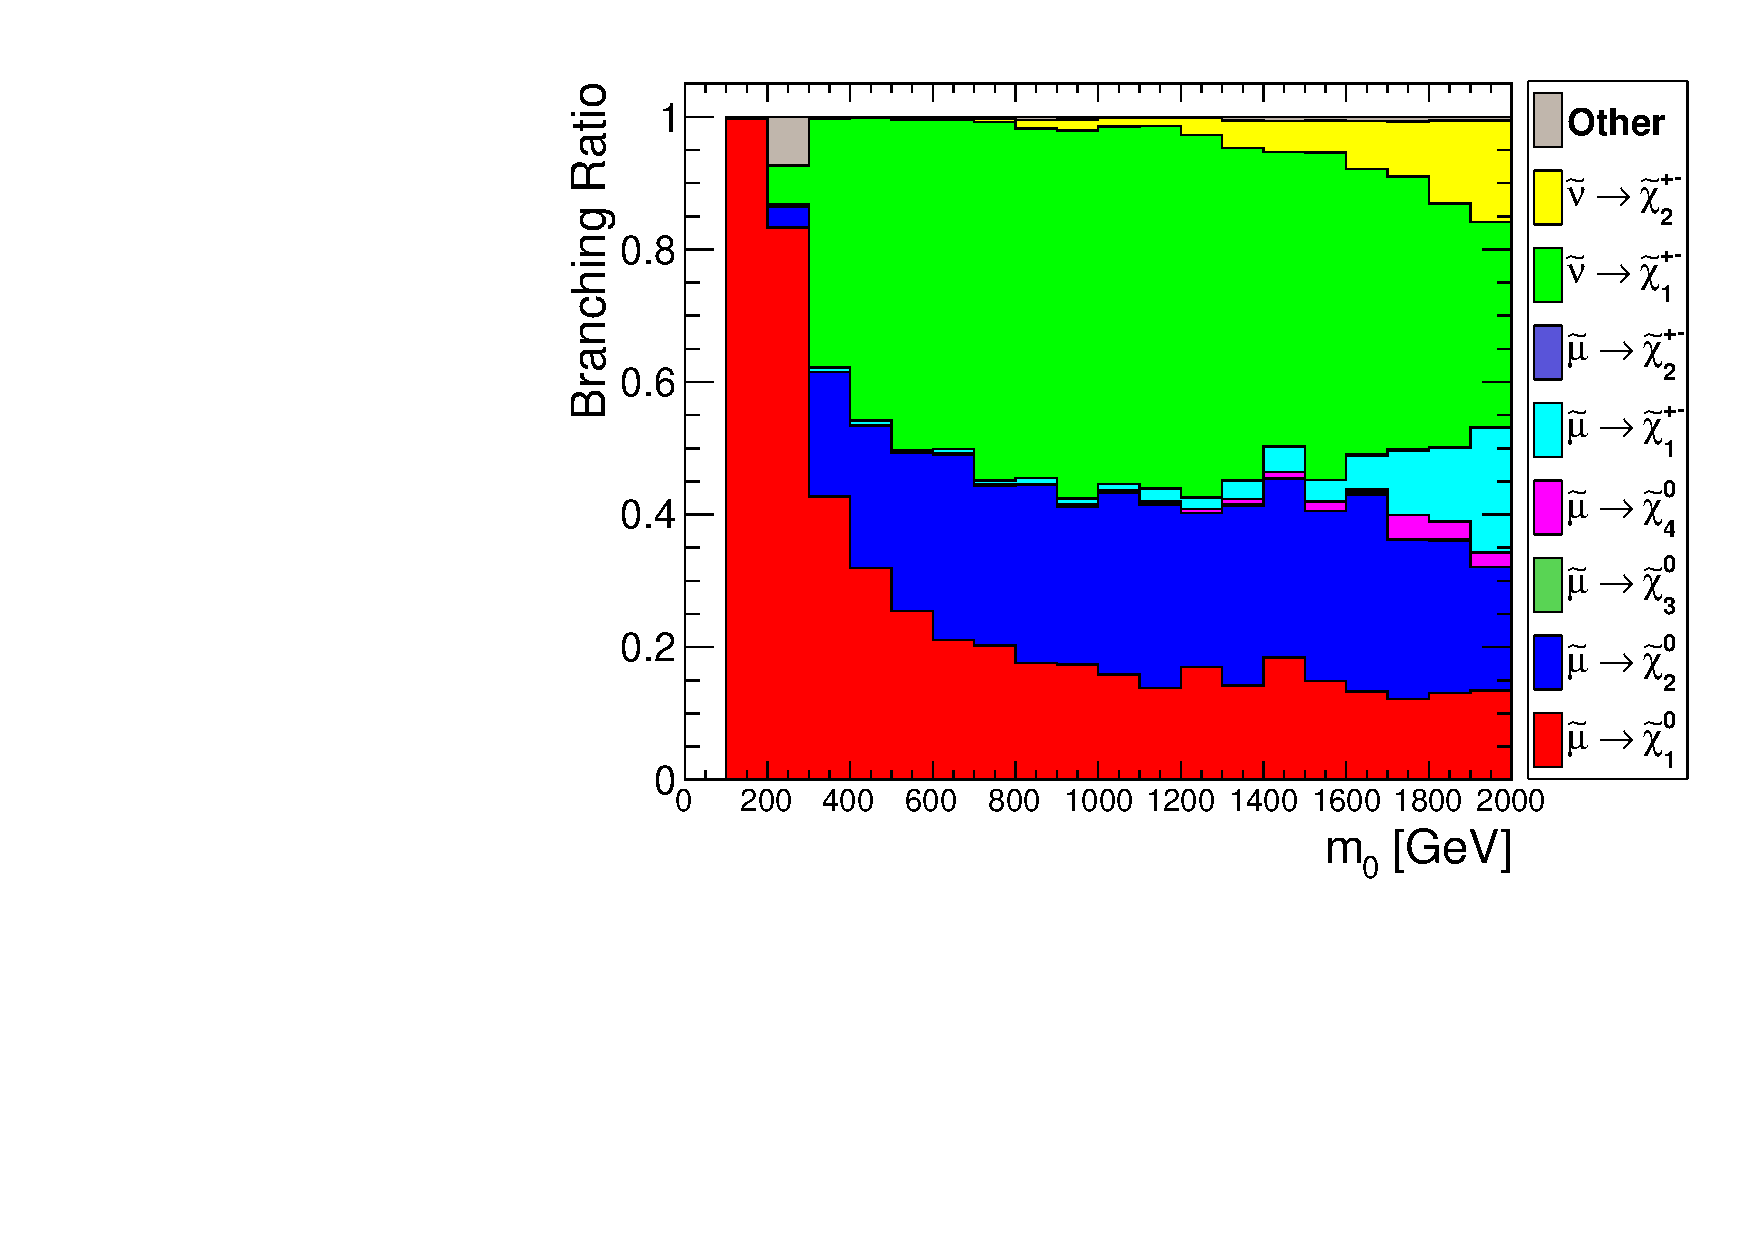
\includegraphics[width=\textwidth]{plots/hCutCrossRatio550.pdf}
    \caption{$m_{1/2} = 550\,\text{GeV}$\label{fig:cutcrossratio550}}
  \end{subfigure}

  \begin{subfigure}[b]{0.495\textwidth}
    \centering
    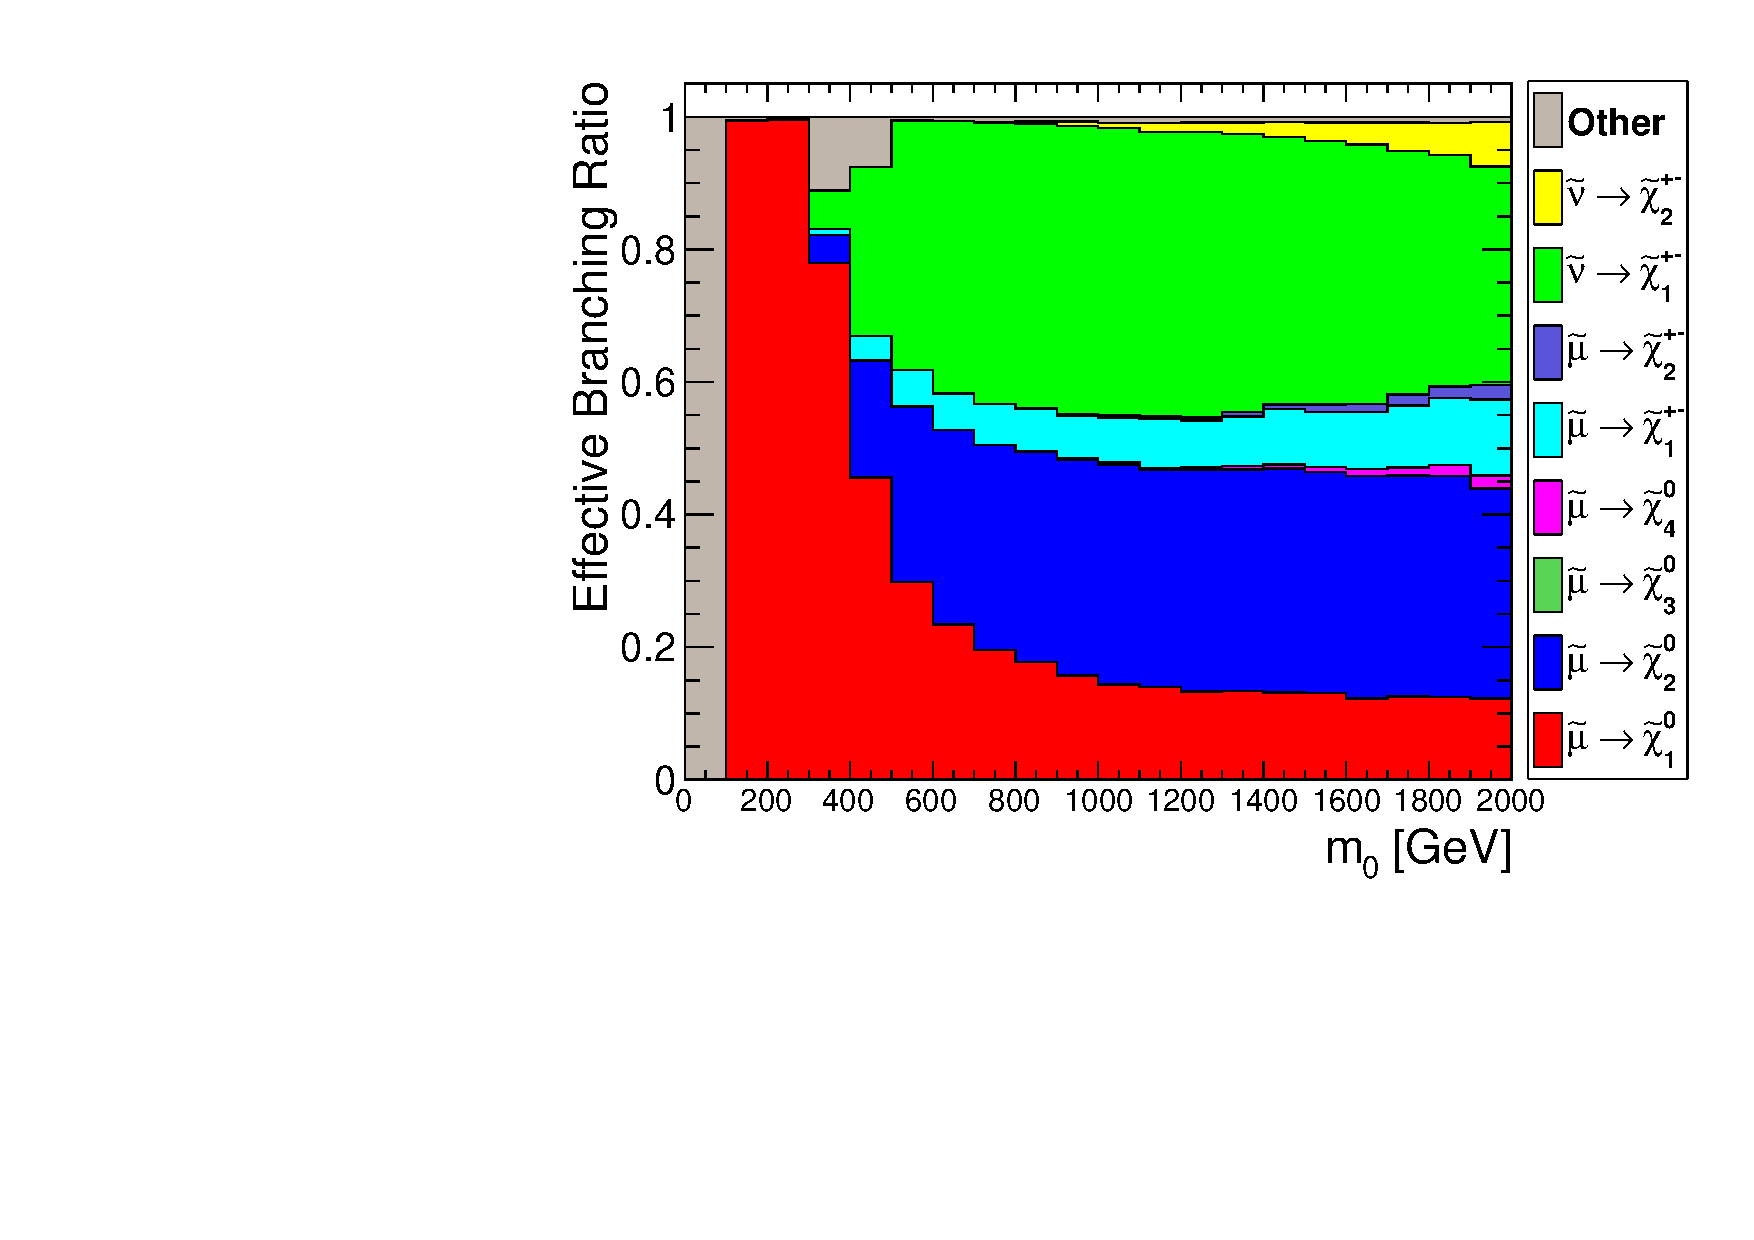
\includegraphics[width=\textwidth]{plots/hCrossRatio750.pdf}
    \caption{$m_{1/2} = 750\,\text{GeV}$\label{fig:crossratio750}}
  \end{subfigure}
  \begin{subfigure}[b]{0.495\textwidth}
    \centering
    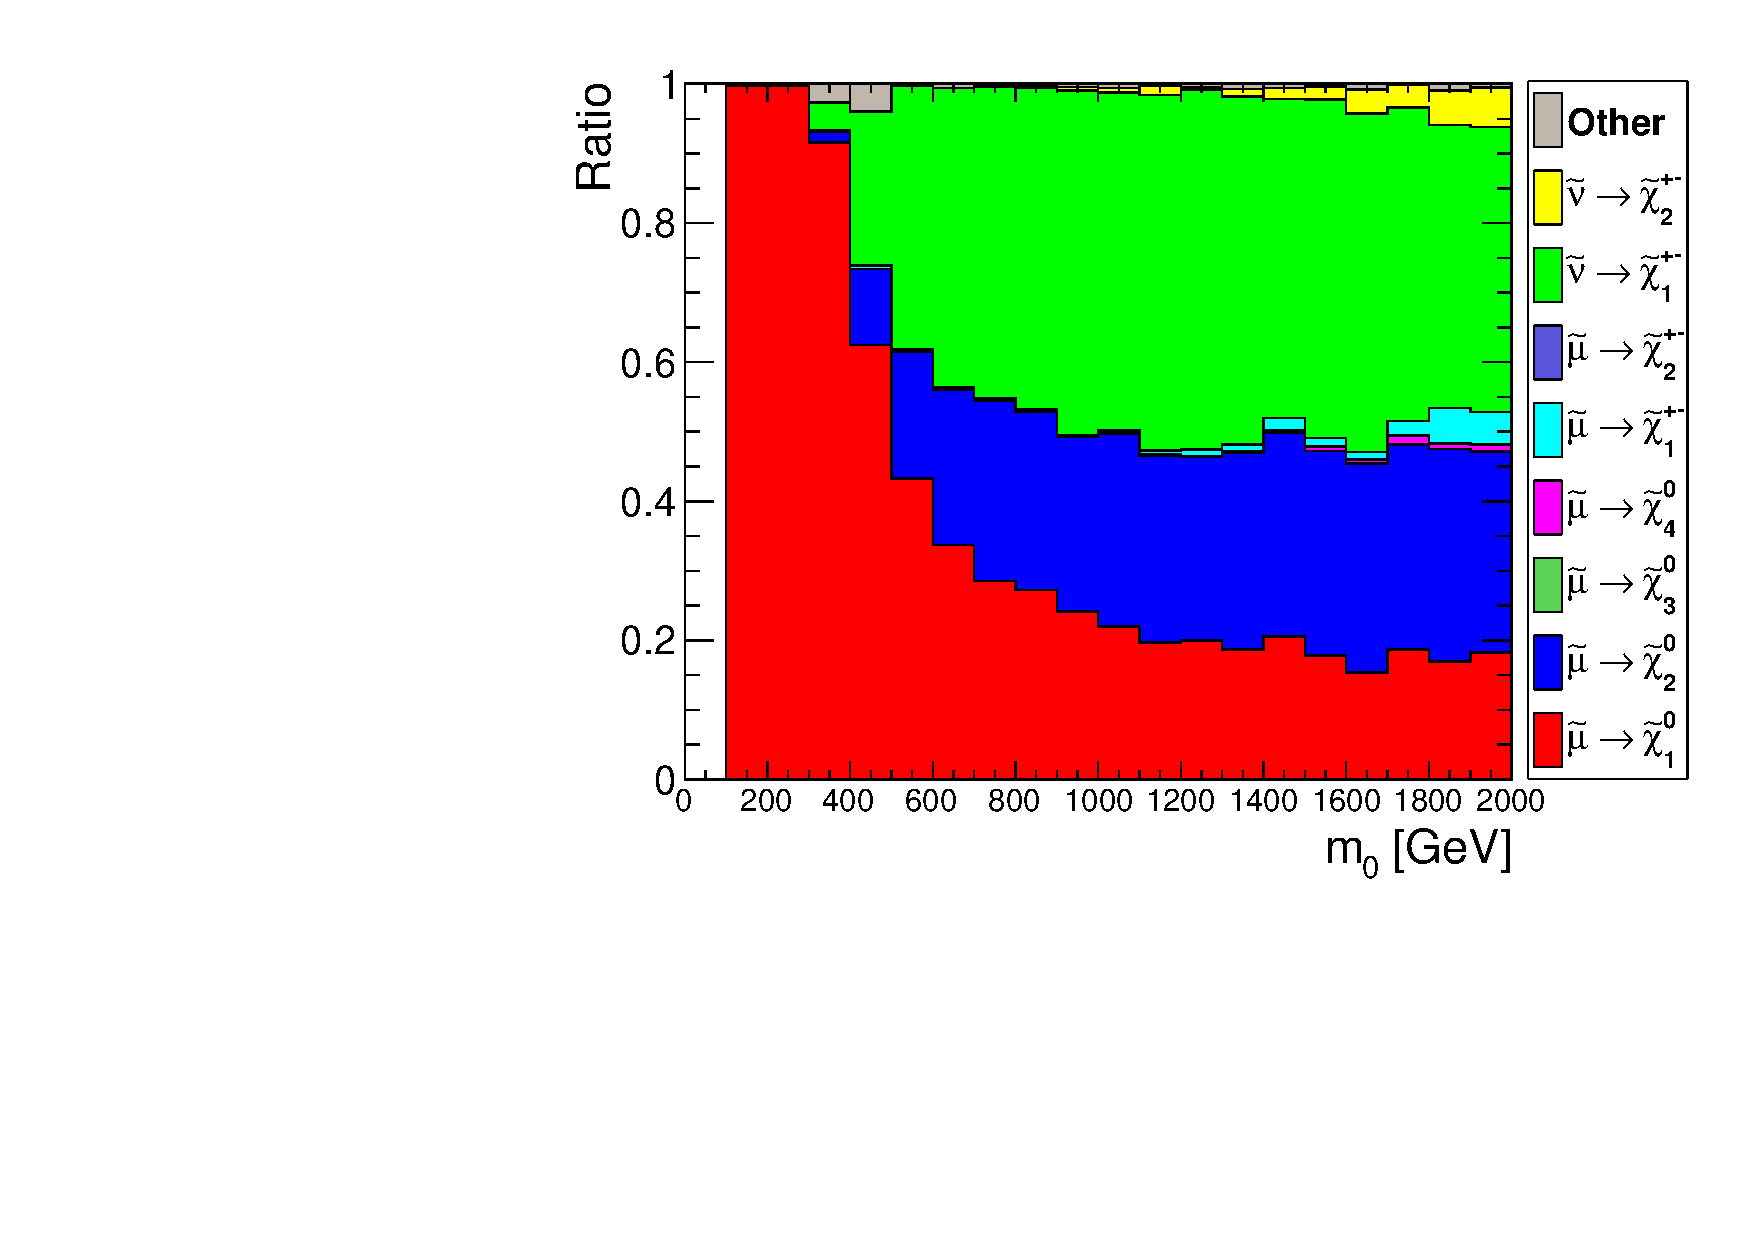
\includegraphics[width=\textwidth]{plots/hCutCrossRatio750.pdf}
    \caption{$m_{1/2} = 750\,\text{GeV}$\label{fig:cutcrossratio750}}
  \end{subfigure}

  \caption{Contributions to the selected signal(-like) events from figure~\ref{fig:sigeff} are shown for fixed values of $m_{1/2}$. All distributions on the left show the MU2J2 case, while the ANA case is given on the right side. Each color represents the relative contribution from a different process, normalized to the respective bin content from~\ref{fig:sigeff}.}
  \label{fig:crossratios}
\end{figure}

Taking the empty bins into account (c.f.~\ref{fig:sigeff}), $550\,\text{GeV}$ as a value for $m_{1/2}$ provides a reasonable overview shown in figures~\ref{fig:crossratio550} and \ref{fig:cutcrossratio550}. To ensure a similar behaviour over the entire $m_{1/2}$ range, two variations with a $200\,\text{GeV}$ difference in the value of $m_{1/2}$ are used for confirmation (Fig.~\ref{fig:crossratio350},~\ref{fig:cutcrossratio350},~\ref{fig:crossratio750} and \ref{fig:cutcrossratio750}). With the grey colour marking the remaining contribution not covered by the listed processes, only a negligible amount is left over. Initially, this statement would contradict the first bin of the MU2J2 case. However, since a ratio is being shown, this can be explained by the very low number of selected events in this region (c.f.~\ref{fig:sigeff}). The ANA case supports this explanation, as none of the events pass its requirements.

As one would expect, for higher sfermion masses the contribution from processes with heavier sparticles increases. However the conclusion that can be drawn from these distributions, is that three processes dominate the signature of this analysis' signal. This is only enhanced by transitioning from the MU2J2, to the ANA case. The corresponding Feynman graphs for each of the three processes are given in figure~\ref{fig:domprocesses}.

\begin{figure}[htb!]
  \centering
  \begin{subfigure}[b]{0.495\textwidth}
    \centering
    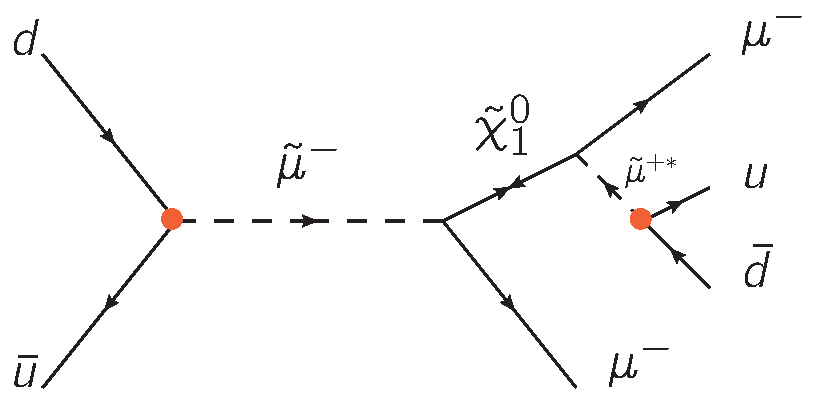
\includegraphics[width=\textwidth]{plots/rpv-resonant-smuon-samesign-mumuqq.pdf}
    \caption{\label{fig:resosmuneut1}}
  \end{subfigure}
  \begin{subfigure}[b]{0.495\textwidth}
    \centering
    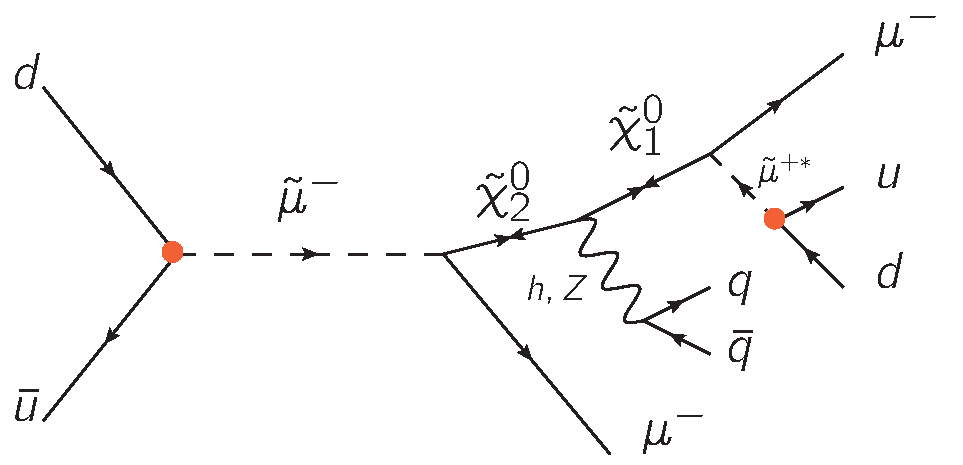
\includegraphics[width=\textwidth]{plots/rpv-resonant-smuon-neutralino2.pdf}
    \caption{\label{fig:resosmuneut2}}
  \end{subfigure}

  \begin{subfigure}[b]{0.495\textwidth}
    \centering
    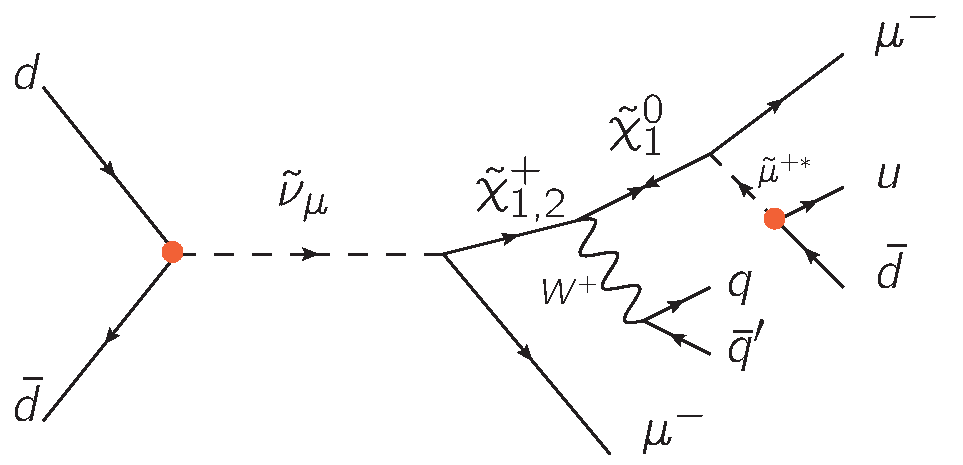
\includegraphics[width=\textwidth]{plots/rpv-resonant-sneutrino-chargino-mumuqq.pdf}
    \caption{\label{fig:resosneutcharg1}}
  \end{subfigure}

  \caption{Feynman graphs of the three dominant processes that lead to the signal signature. Each of the cascades leads to the neutralino LSP, which then decays through the $\lambda^\prime_{211}$ coupling, adding two jets and one muon to the final state.}
  \label{fig:domprocesses}
\end{figure}

\noindent As mentioned beforehand, after reaching the LSP through the cascade, the decay through the $\lambda^\prime_{211}$ leading to two jets and one muon is identical for every process. The most simple graph (Fig.~\ref{fig:resosmuneut1}) has its biggest contribution of up to almost $100\pct$ in the low $m_0$ region. It then quickly loses importance and remains at a constant level around $20\pct$. Both the other processes gain importance as the simple one loses it. Their contribution levels around $25\pct$ for the $\tilde{\mu} \rightarrow \tilde{\chi}^0_2$ and $45\pct$ for the $\tilde{\nu} \rightarrow \tilde{\chi}^\pm_1$ process for $500\,\text{GeV} < m_0 < 1600\,\text{GeV}$. Afterwards they decrease slowly.

This information can be used to allow for different interpretations of the results of this analysis. In addition to using the supersymmetric model, simplified models for the three Feynman graphs are an option. Since these types of models only focus on the physical parameters such as the particle mass and coupling strengths, it is easier to extrapolate from the results when working with different assumptions.



%%% Local Variables: 
%%% mode: latex
%%% TeX-master: "document"
%%% End: 
